\documentclass[10pt]{article}
\usepackage[a4paper,margin=18mm]{geometry}
\usepackage[T1]{fontenc}\usepackage{lmodern}
\usepackage{amsmath,amssymb,booktabs,array,enumitem}
\usepackage{tikz}\usetikzlibrary{shapes.gates.logic.US,positioning,arrows.meta}
\usepackage[hidelinks]{hyperref}
\setlength{\parindent}{0pt}\setlength{\parskip}{4pt}\setlength{\emergencystretch}{2em}
\newcommand{\mos}[4]{\begin{scope}[shift={(#1,#2)}]
\draw(0,.24)--(0,-.24);\draw(0,.2)--(.25,.2)--(.25,.5);\draw(0,-.2)--(.25,-.2)--(.25,-.5);
\draw(-.16,.23)--(-.16,-.23);
\ifnum#4=1\draw(-.26,0)circle(.06);\draw(-.75,0)--(-.32,0);\else\draw(-.75,0)--(-.16,0);\fi
\node[anchor=east,font=\scriptsize]at(-.76,0){$#3$};\end{scope}}
\newcommand{\gnd}[2]{\draw(#1,#2)--(#1,{#2-.12});\draw({#1-.17},{#2-.12})--({#1+.17},{#2-.12});\draw({#1-.11},{#2-.2})--({#1+.11},{#2-.2});}
\newcommand{\rail}[3]{\draw(#1,#2)--(#1,{#2+.14});\node[above,font=\scriptsize]at(#1,{#2+.14}){$#3$};}
\begin{document}
\begin{center}{\Large EE3032 Introduction to VLSI Design---Final}\\Fall 2009\end{center}
Reconstructed from the complete three-page original (printed pages 1-1 through 1-3). The seven printed question weights sum to \textbf{90\%}; no missing 10\% question is invented. Source wording, the full overbar in Q7, and all transistor/clock polarities are preserved. All figures are editable TikZ, including paths from the native vector layout.\par\medskip
\textbf{1. (15\%)} Figure 1 shows a circuit for realizing a low-cost latch. Complete the following questions.
\begin{enumerate}[label=(\alph*)]
\item What type of latch is realized by the circuit? (5\%)
\item Assume that the switching threshold voltage of the inverter Inv1 is $V_{dd}/2$. List two inequalities for determining the sizes of P2 and N2. (10\%)
\end{enumerate}\begin{center}\begin{tikzpicture}[scale=.8,font=\small]
\mos{0}{4.8}{}{1}\mos{0}{3.4}{}{0}\rail{.25}{5.3}{V_{DD}}\draw(.25,4.3)--(.25,3.9);\gnd{.25}{2.9}
\mos{0}{1.7}{D}{1}\mos{0}{.3}{D}{0}\rail{.25}{2.2}{V_{DD}}\draw(.25,1.2)--(.25,.8);\gnd{.25}{-.2}\node[right]at(.45,1.7){P1};\node[right]at(.45,.3){N1};
\draw(.25,1)--(2.1,1);\draw(2.1,.78)rectangle(2.5,1.22);\draw(2.3,1.22)--(2.3,1.52);\draw(2.3,1.58)circle(.06);\draw(.25,4.1)--(2.3,4.1)--(2.3,1.64);
\draw(2.3,.78)--(2.3,-.8)--(-1.6,-.8)--(-1.6,4.8)--(-.75,4.8);\draw(-1.6,3.4)--(-.75,3.4);\draw(-1.6,4.1)--(-2.25,4.1)node[left]{CLK};\fill(-1.6,4.1)circle(1.5pt);
\mos{5}{1.7}{}{1}\mos{5}{.3}{}{0}\rail{5.25}{2.2}{V_{DD}}\draw(5.25,1.2)--(5.25,.8);\gnd{5.25}{-.2}
\draw(2.5,1)--(3.8,1)--(3.8,.3)--(4.25,.3);\draw(3.8,1.7)--(4.25,1.7);\draw(3.8,.3)--(3.8,1.7);\fill(3.8,1)circle(1.5pt);\draw[dashed](4.05,-.45)rectangle(5.65,2.7);\node[above]at(4.9,2.7){Inv1};
\draw(5.25,1)--(7.8,1)node[right]{Q};\fill(6.85,1)circle(1.5pt);
\begin{scope}[shift={(5.5,-1.6)},xscale=-1]\mos{0}{0}{}{1}\end{scope}\begin{scope}[shift={(5.5,-3)},xscale=-1]\mos{0}{0}{}{0}\end{scope}\rail{5.25}{-1.1}{V_{DD}}\draw(5.25,-2.1)--(5.25,-2.5);\gnd{5.25}{-3.5}\node[above]at(5.6,-1.35){P2};\node[above]at(5.6,-2.75){N2};
\draw(6.85,1)--(6.85,-3)--(6.25,-3);\draw(6.85,-1.6)--(6.25,-1.6);\draw(3.8,1)--(3.8,-2.3)--(5.25,-2.3);\fill(5.25,-2.3)circle(1.5pt);
\end{tikzpicture}\\Figure 1: A low-cost latch. The feedback pair is always connected.\end{center}\newpage\textbf{2. (15\%)} Explain the operation principle of the circuit shown in Figure 2 shows a circuit for realizing a dynamic register. Answer the following questions.
\begin{enumerate}[label=(\alph*)]
\item Explain the operation principle of the circuit. (5\%)
\item Design the register using the static low-cost latches shown in Figure 1. (10\%)
\end{enumerate}\begin{center}\begin{tikzpicture}[scale=.9,font=\small]
\foreach \x in {0,3,6,9}{\rail{\x+.25}{4}{V_{DD}}\gnd{\x+.25}{.2}}
\mos{0}{3.5}{}{1}\mos{0}{2.1}{\phi}{0}\mos{0}{.7}{}{0}\draw(.25,3)--(.25,2.6);\draw(.25,1.6)--(.25,1.2);
\mos{3}{3.5}{}{1}\mos{3}{2.1}{\phi}{0}\mos{3}{.7}{}{0}\draw(3.25,3)--(3.25,2.6);\draw(3.25,1.6)--(3.25,1.2);
\mos{6}{3.5}{}{1}\mos{6}{2.1}{\phi}{1}\mos{6}{.7}{}{0}\draw(6.25,3)--(6.25,2.6);\draw(6.25,1.6)--(6.25,1.2);
\mos{9}{3.5}{}{1}\mos{9}{2.1}{\phi}{1}\mos{9}{.7}{}{0}\draw(9.25,3)--(9.25,2.6);\draw(9.25,1.6)--(9.25,1.2);
\draw(-.75,3.5)--(-1.3,3.5)--(-1.3,.7)--(-.75,.7);\draw(-1.3,2.8)--(-2,2.8)node[left]{$I$};\draw(.25,2.8)--(1.7,2.8)--(1.7,3.5)--(2.25,3.5);\draw(1.7,2.8)--(1.7,.7)--(2.25,.7);\node[above]at(.8,2.8){$A$};\fill(1.7,2.8)circle(1.5pt);
\draw(3.25,2.8)--(4.7,2.8)--(4.7,3.5)--(5.25,3.5);\draw(4.7,2.8)--(4.7,.7)--(5.25,.7);\node[above]at(3.9,2.8){$B$};\fill(4.7,2.8)circle(1.5pt);
\draw(6.25,1.4)--(7.7,1.4)--(7.7,3.5)--(8.25,3.5);\draw(7.7,1.4)--(7.7,.7)--(8.25,.7);\node[below]at(6.9,1.4){$C$};\fill(7.7,1.4)circle(1.5pt);\draw(9.25,1.4)--(11,1.4)node[right]{$O$};
\end{tikzpicture}\\Figure 2: A dynamic CMOS register circuit. All four three-device stages and the two clock-controlled pMOS bubbles are retained.\end{center}\textbf{3. (10\%)} Complete the following questions.
\begin{enumerate}[label=(\alph*)]
\item Figure 3(a) shows a three-input dynamic logic gate. Assume that the sizes of the NMOS and PMOS transistors of the dynamic logic gate and the inverter are equal and $C_g/C_d=\alpha$ ($C_d=C_s$). Also, the threshold voltage of the inverter is $V_{dd}/2$. Derive the minimal value of $\alpha$ such that the circuit can work correctly. (5\%)
\item Complete the restore circuit of Figure 3(b), such that $Y=0$ when $X=0$ and $C=0$. (5\%)
\end{enumerate}\begin{center}\begin{tikzpicture}[scale=.8,font=\small]
\mos{0}{5.6}{}{1}\rail{.25}{6.1}{V_{dd}}\draw(.25,5.1)--(.25,4.7);\draw(-.75,5.6)--(-1.9,5.6)--(-1.9,0)--(-.75,0);\draw(-1.9,3)--(-2.5,3)node[left]{$V_{in}$};
\foreach \y in {4.2,2.8,1.4}{\mos{0}{\y}{}{0}}
\mos{0}{0}{}{0}\draw(.25,3.7)--(.25,3.3);\draw(.25,2.3)--(.25,1.9);\draw(.25,.9)--(.25,.5);\gnd{.25}{-.5}
\foreach \y in {3.5,2.1,.7}{\draw(.25,\y)--(1.3,\y)--(1.3,\y-.2);\draw(1.1,\y-.2)--(1.5,\y-.2);\draw(1.1,\y-.32)--(1.5,\y-.32);\draw(1.3,\y-.32)--(1.3,\y-.55);\gnd{1.3}{\y-.55}}
\node[not gate US,draw](i)at(3,4.95){};\draw(.25,4.95)--(i.input);\draw(i.output)--(4,4.95);\node[above]at(1.5,4.95){$V_F$};\node at(.6,-1){(a)};
\begin{scope}[xshift=6cm,yshift=2.4cm]
\draw(0,0)--(1.1,0)node[pos=0,left]{$X$};\draw(1.1,-.16)rectangle(1.55,.16);\draw(1.32,-.16)--(1.32,-.42);\draw(1.32,-.48)circle(.06);\draw(1.32,-.54)--(1.32,-.95)node[below]{$C$};\draw(1.55,0)--(2.7,0)node[midway,above]{$Y$};\draw[dashed](2.7,-.5)rectangle(4.3,.5);\node[align=center]at(3.5,0){restore\\circuit};\draw(4.3,0)--(4.9,0);\node at(2,-2.1){(b)};\end{scope}
\end{tikzpicture}\\Figure 3: (a) Dynamic logic. (b) Pass-transistor design. The unlabelled three data gates in (a) are preserved.\end{center}\newpage\textbf{4. (15\%)} Figure 4 shows a circuit designed with NP-domino logic. Complete the following questions.
\begin{enumerate}[label=(\alph*)]
\item What function does this circuit realize? (5\%)
\item Using timing diagrams, describe the operation of the circuit. (5\%)
\item Design the circuit using Domino logic. (5\%)
\end{enumerate}\begin{center}\begin{tikzpicture}[scale=.75,font=\small]
\mos{0}{3.6}{\phi}{1}\rail{.25}{4.1}{V_{DD}}\draw(.25,3.1)--(.25,2.6);\draw(-1.75,2.6)--(2.25,2.6);\fill(.25,2.6)circle(1.5pt);
\mos{-2}{1.8}{A}{0}\mos{-2}{.4}{B}{0}\draw(-1.75,2.6)--(-1.75,2.3);\draw(-1.75,1.3)--(-1.75,.9);
\mos{1}{1.8}{C}{0}\draw(1.25,2.6)--(1.25,2.3);\draw(1.25,1.3)--(1.25,1.1);\draw(.25,1.1)--(2.25,1.1);\mos{0}{.4}{A}{0}\mos{2}{.4}{B}{0}\draw(.25,1.1)--(.25,.9);\draw(2.25,1.1)--(2.25,.9);
\draw(-1.75,-.1)--(-1.75,-.4)--(2.25,-.4)--(2.25,-.1);\draw(.25,-.1)--(.25,-.8);\fill(.25,-.4)circle(1.5pt);\mos{0}{-1.3}{\phi}{0}\gnd{.25}{-1.8}
\node[not gate US,draw,rotate=-90](ix)at(3.5,1.2){};\draw(2.25,2.6)--(3.5,2.6)--(ix.input);\draw(ix.output)--(3.5,.15)node[below]{$X$};
\mos{8}{3.9}{\bar\phi}{1}\rail{8.25}{4.4}{V_{DD}}\draw(8.25,3.4)--(8.25,3.1);\draw(6.25,3.1)--(10.25,3.1);\mos{6}{2.4}{A}{1}\mos{8}{2.4}{B}{1}\mos{10}{2.4}{C}{1}
\foreach \x in {6.25,8.25,10.25}{\draw(\x,3.1)--(\x,2.9);\draw(\x,1.9)--(\x,1.6);}\draw(6.25,1.6)--(10.25,1.6);
\mos{6}{.7}{}{1}\mos{10}{.7}{A}{1}\mos{10}{-.7}{B}{1}\mos{10}{-2.1}{C}{1}\draw(6.25,1.6)--(6.25,1.2);\draw(10.25,1.6)--(10.25,1.2);\draw(10.25,.2)--(10.25,-.2);\draw(10.25,-1.2)--(10.25,-1.6);
\draw(6.25,.2)--(6.25,-3)--(10.25,-3)--(10.25,-2.6);\draw(8.25,-3)--(8.25,-3.35);\mos{8}{-3.85}{\bar\phi}{0}\gnd{8.25}{-4.35}
\draw(2.25,2.6)--(4.6,2.6)--(4.6,.7)--(5.25,.7);\fill(3.5,2.6)circle(1.5pt);\node[not gate US,draw,rotate=-90](iy)at(11.7,-3.25){};\draw(10.25,-3)--(11.7,-3)--(iy.input);\draw(iy.output)--(11.7,-4.2)node[below]{$Y$};
\end{tikzpicture}\\Figure 4: A circuit designed with NP-domino logic. The static output inverters X and Y are retained.\end{center}\textbf{5. (10\%)} Figure 5 shows a sequential circuit (pipelined circuit). Assume that your boss asks you to design the circuit such that the circuit can be operated at $200\,MHz$. Also, assume that the clock-to-Q propagation delay, the clock-to-Q contamination delay, the setup time, and the hold time of registers R1 and R2 are $0.5\,ns$, $0.2\,ns$, $1.5\,ns$, and $1\,ns$, respectively. Determine the maximum and minimum delays of the combinational circuit.\begin{center}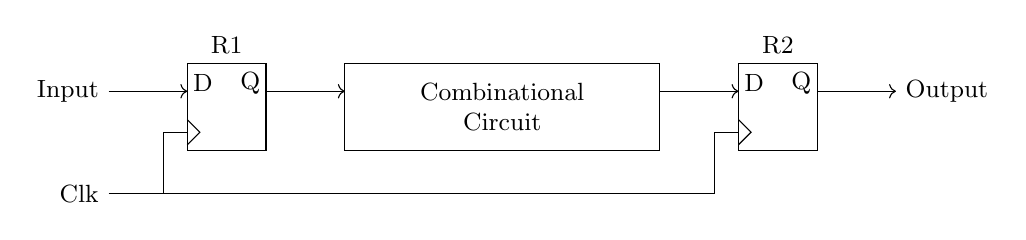
\begin{tikzpicture}[font=\small]
\foreach \x/\name in {0/R1,7/R2}{\draw(\x,-.45)rectangle(\x+1,.65);\node at(\x+.2,.4){D};\node at(\x+.8,.4){Q};\draw(\x,-.38)--(\x+.16,-.22)--(\x,-.06);\node[above]at(\x+.5,.65){\name};\draw(\x-.3,-1)--(\x-.3,-.22)--(\x,-.22);}
\draw(2,.65)rectangle(6,-.45);\node[align=center]at(4,.1){Combinational\\Circuit};\draw[->](-1,.3)--(0,.3);\node[left]at(-1,.3){Input};\draw[->](1,.3)--(2,.3);\draw[->](6,.3)--(7,.3);\draw[->](8,.3)--(9,.3)node[right]{Output};\draw(-1,-1)--(6.7,-1);\node[left]at(-1,-1){Clk};
\end{tikzpicture}\\Figure 5: A pipelined circuit.\end{center}\newpage\textbf{6. (10\%)} Figure 6 shows the symbolic layout of a circuit. Draw the transistor-level schematic diagram of the circuit.\begin{center}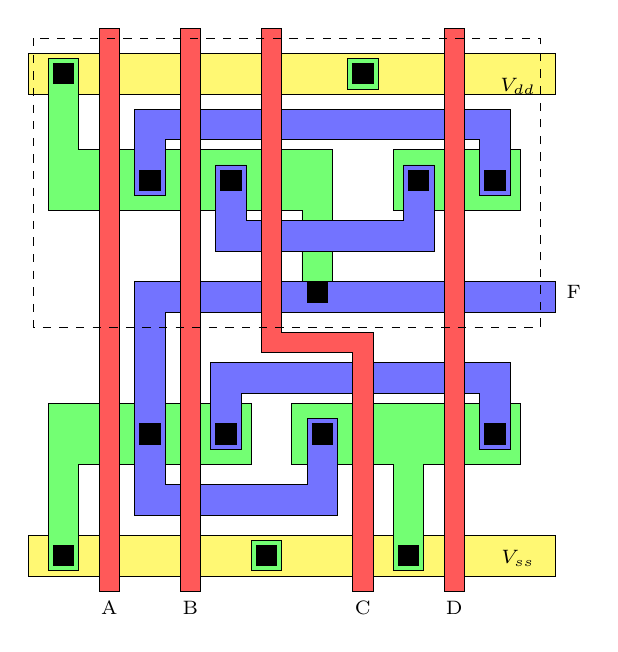
\begin{tikzpicture}[x=.038cm,y=-.038cm,font=\scriptsize]
\draw[fill=yellow!55,line width=.25pt](1.26400,9.12480)--(177.61200,9.12480)--(177.61200,22.69000)--(1.26400,22.69000)--cycle;
\draw[fill=yellow!55,line width=.25pt](1.26400,170.21180)--(177.61200,170.21180)--(177.61200,183.77700)--(1.26400,183.77700)--cycle;
\draw[fill=green!55,line width=.25pt](123.35100,41.34230)--(165.74240,41.34230)--(165.74240,61.69000)--(123.35100,61.69000)--cycle;
\draw[fill=green!55,line width=.25pt](75.87200,171.90820)--(86.04620,171.90820)--(86.04620,182.08200)--(75.87200,182.08200)--cycle;
\draw[fill=green!55,line width=.25pt](108.09000,10.82120)--(118.26380,10.82120)--(118.26380,20.99500)--(108.09000,20.99500)--cycle;
\draw[fill=green!55,line width=.25pt](8.04600,182.08200)--(18.22000,182.08200)--(18.22000,146.47300)--(75.87200,146.47300)--(75.87200,126.12500)--(8.04600,126.12500)--(8.04600,182.08200)--cycle;
\draw[fill=green!55,line width=.25pt](165.74200,126.12500)--(89.43800,126.12500)--(89.43800,146.47300)--(123.35100,146.47300)--(123.35100,182.08200)--(133.52500,182.08200)--(133.52500,146.47300)--(165.74200,146.47300)--(165.74200,126.12500)--cycle;
\draw[fill=green!55,line width=.25pt](8.04600,10.82100)--(18.22000,10.82100)--(18.22000,41.34300)--(103.00300,41.34300)--(103.00300,93.90800)--(92.82900,93.90800)--(92.82900,61.69000)--(8.04600,61.69000)--(8.04600,10.82100)--cycle;
\draw[fill=blue!55,line width=.25pt](94.52500,131.21200)--(104.69800,131.21200)--(104.69800,163.43000)--(36.87300,163.43000)--(36.87300,85.43000)--(177.61200,85.43000)--(177.61200,95.60400)--(47.04600,95.60400)--(47.04600,153.25500)--(94.52500,153.25500)--(94.52500,131.21200)--cycle;
\draw[fill=blue!55,line width=.25pt](62.30700,141.38600)--(72.48100,141.38600)--(72.48100,122.73400)--(152.17700,122.73400)--(152.17700,141.38600)--(162.35100,141.38600)--(162.35100,112.56000)--(62.30700,112.56000)--(62.30700,141.38600)--cycle;
\draw[fill=blue!55,line width=.25pt](36.87300,56.60400)--(47.04600,56.60400)--(47.04600,37.95100)--(152.17700,37.95100)--(152.17700,56.60400)--(162.35100,56.60400)--(162.35100,27.77700)--(36.87300,27.77700)--(36.87300,56.60400)--cycle;
\draw[fill=blue!55,line width=.25pt](64.00300,46.43000)--(74.17700,46.43000)--(74.17700,65.08200)--(126.74200,65.08200)--(126.74200,46.43000)--(136.91600,46.43000)--(136.91600,75.25500)--(64.00300,75.25500)--(64.00300,46.43000)--cycle;
\draw[fill=red!65,line width=.25pt](52.13300,0.64600)--(58.91581,0.64600)--(58.91581,188.86400)--(52.13300,188.86400)--cycle;
\draw[fill=red!65,line width=.25pt](25.00300,0.64600)--(31.78581,0.64600)--(31.78581,188.86400)--(25.00300,188.86400)--cycle;
\draw[fill=red!65,line width=.25pt](140.30700,0.64600)--(147.08981,0.64600)--(147.08981,188.86400)--(140.30700,188.86400)--cycle;
\draw[fill=red!65,line width=.25pt](79.26400,0.64700)--(79.26400,109.16900)--(109.78600,109.16900)--(109.78600,188.86400)--(116.56800,188.86400)--(116.56800,102.38600)--(86.04600,102.38600)--(86.04600,0.64700)--(79.26400,0.64700)--cycle;
\draw[fill=black,line width=.25pt](9.74200,173.60358)--(16.52442,173.60358)--(16.52442,180.38600)--(9.74200,180.38600)--cycle;
\draw[fill=black,line width=.25pt](125.04600,173.60358)--(131.82842,173.60358)--(131.82842,180.38600)--(125.04600,180.38600)--cycle;
\draw[fill=black,line width=.25pt](153.87200,132.90758)--(160.65481,132.90758)--(160.65481,139.69000)--(153.87200,139.69000)--cycle;
\draw[fill=black,line width=.25pt](64.00300,132.90758)--(70.78581,132.90758)--(70.78581,139.69000)--(64.00300,139.69000)--cycle;
\draw[fill=black,line width=.25pt](9.74200,12.51619)--(16.52442,12.51619)--(16.52442,19.29900)--(9.74200,19.29900)--cycle;
\draw[fill=black,line width=.25pt](38.56800,48.12519)--(45.35081,48.12519)--(45.35081,54.90800)--(38.56800,54.90800)--cycle;
\draw[fill=black,line width=.25pt](153.87200,48.12519)--(160.65481,48.12519)--(160.65481,54.90800)--(153.87200,54.90800)--cycle;
\draw[fill=black,line width=.25pt](128.43800,48.12519)--(135.22081,48.12519)--(135.22081,54.90800)--(128.43800,54.90800)--cycle;
\draw[fill=black,line width=.25pt](65.69800,48.12519)--(72.48081,48.12519)--(72.48081,54.90800)--(65.69800,54.90800)--cycle;
\draw[fill=black,line width=.25pt](94.52500,85.42958)--(101.30781,85.42958)--(101.30781,92.21200)--(94.52500,92.21200)--cycle;
\draw[fill=black,line width=.25pt](96.22000,132.90758)--(103.00242,132.90758)--(103.00242,139.69000)--(96.22000,139.69000)--cycle;
\draw[fill=black,line width=.25pt](38.56800,132.90758)--(45.35081,132.90758)--(45.35081,139.69000)--(38.56800,139.69000)--cycle;
\draw[fill=black,line width=.25pt](109.78600,12.51619)--(116.56842,12.51619)--(116.56842,19.29900)--(109.78600,19.29900)--cycle;
\draw[fill=black,line width=.25pt](77.56800,173.60358)--(84.35081,173.60358)--(84.35081,180.38600)--(77.56800,180.38600)--cycle;
\draw[dashed](2.959,4.038)rectangle(172.524,100.69);
\node[right]at(178,88.82){F};\node at(165,20){$V_{dd}$};\node at(165,178){$V_{ss}$};
\node[below]at(28.4,188.864){A};\node[below]at(55.52,188.864){B};\node[below]at(113.18,188.864){C};\node[below]at(143.7,188.864){D};
\end{tikzpicture}\\Figure 6: The symbolic layout. Editable native path coordinates: green diffusion, yellow Metal 2, blue Metal 1, red poly, black contact; dashed n-well. Crossings without black contacts do not connect layers.\end{center}\textbf{7. (15\%)} Sketch the Boolean function $f=\overline{AB+C+DE}$ using each of the following circuit techniques. (1) Domino logic (5\%) (2) Fully differential logic (5\%) (3) Static CMOS logic (5\%).\end{document}